% This sample file is dedicated to the public domain.
\chapter{Experimental measurement system and procedures}
\label{chap.experimental}

\section{Overview}

Thus far we have considered flux noise in SQUIDs and qubits in a theoretical context. However, the bulk of our work is concerned with the experimental characterization of flux noise in SQUIDs. The success of this endeavor relies on a robust experimental measurement system that satisfies a number of stringent requirements. First and foremost, because we seek to accurately measure the intrinsic noise in SQUIDs, which are themselves ultra-low-noise devices, every care must be taken to insure that the measurement system produces as little noise as possible. In this same thread, $1/f$-noise measurements at low frequencies are necessarily slow measurements, which entails that the system must be ultra-stable over time scales on the order of hours. As noise originating from myriad sources---electronic and mechanical as well as temperature and magnetic field fluctuations, for example---can couple into the measurement, the design considerations are considerable.

We also seek to characterize the flux noise as a function of device temperature, which means that we need a refrigeration apparatus that can hold a stable temperature from approximately 0.1~K up to 4~K. Standard dilution refrigerators are quite capable of reaching such temperatures, but we shall see that care is needed to achieve the required stabilities well in excess of 1 part in $10^4$.

For a number of reasons, it is advantageous for the system to have the ability to cool multiple SQUIDs in a single cool-down and to measure each one individually. On one hand, the length of the cool-down and warm-up procedures of our dilution refrigerator means that considerable time is saved over cooling each SQUID individually. On another hand, cooling several SQUIDs at once eliminates many potential confounding factors---trapped magnetic fields, for example---that could conceivably cause differences between measurements from different cool-downs.

In this Chapter we review the experimental design and implementation as well as the validation, calibration, and measurement procedure. The main components of the system are the [@@@ probably put the sections here], which we now discuss in detail.

\section{Measurement overview}

\begin{figure}
\centering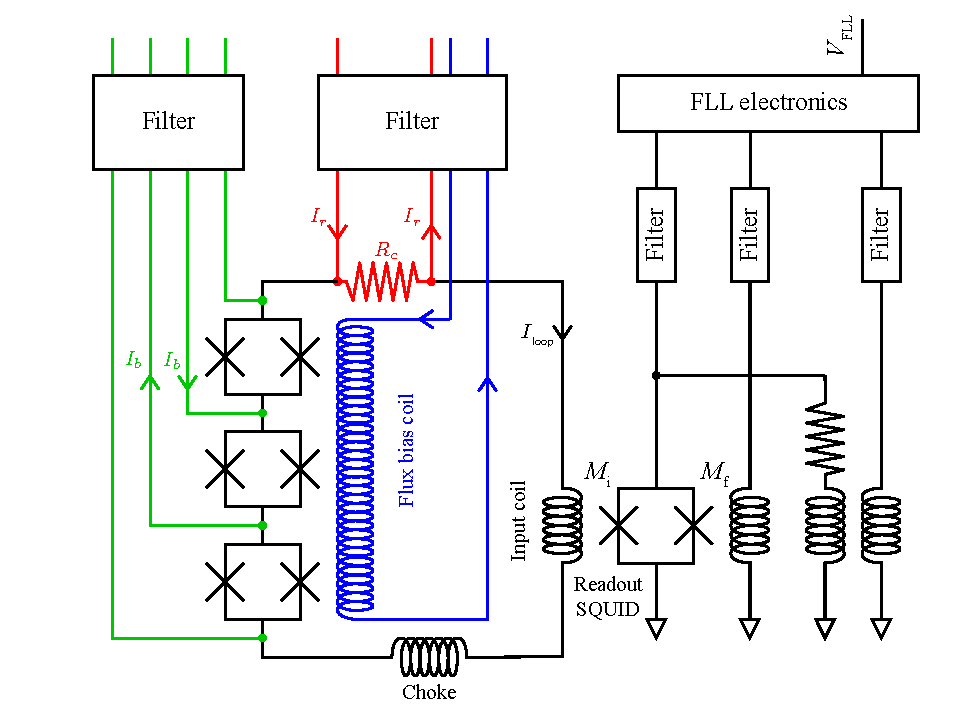
\includegraphics{experimental/Fig_schematic}\\
\caption[Schematic of measurement system]{Configuration of measurement system to measure flux noise in three SQUIDs. The bias current $I_b$ shown enables the measurement of the middle SQUID. The static voltage across the SQUID is canceled by the current $I_r$ applied to the compensating resistor $R_c$. [@@@ transformer ratios]}
\label{fig:experimental:schematic}
\end{figure}

The principle behind our measurement technique is that a SQUID biased into the normal state generates fluctuations based on changes in its critical current and the flux through its loop. Naturally, these fluctuations are quite small and cannot be read directly using even the best room-temperature amplifier. Therefore, we use a second SQUID, operated in a standard flux-locked loop (FLL) configuration, to detect the fluctuations. The fluctuations are monitored for long periods of time, converted to spectral densities, and subsequently analyzed.

The basis of our system is the circuit schematic illustrated in Fig.~\ref{fig:experimental:schematic}, where we have modified the design used by Wellstood~\citep{Wellstood:thesis} in order to accommodate multiple measured SQUIDs. In the circuit, several SQUIDs are connected in series with a small compensating resistor $R_c$, the input coil to the readout SQUID, and a choke inductor, which prevents high-frequency cross-talk between SQUIDs. Appropriate wiring to the circuit allows us to inject currents across the compensating resistor and each of the SQUIDs. To make a measurement, we begin by injecting a current $I_b$ through a particular SQUID and increasing it until the SQUID enters the normal state with voltage $V_{\text{SQUID}}$. At this point, most of the current bias passes through the measured SQUID, but a small amount $\Vsquid/R_c$ is shunted through the compensating resistor. If $I_b$ is increased further, a fraction $R_c/(R_d+R_c)$ passes through the resistor, where $R_d$ is the dynamic resistance of the measured SQUID. For reasons we discuss later, $R_c \ll R_d$ by design. If large enough, the shunted current that flows around the big loop can drive the other SQUIDs normal, where they begin to add their own intrinsic noise. To prevent this, a current $I_r$ is passed through the compensating resistor until $V_{\text{SQUID}} = I_r R_c$ and no net current flows around the loop, ensuring that the SQUIDs not under measurement remain superconducting and contribute no noise.

At this point, a variation in the critical current of the SQUID will redistribute the bias currents to the circuit. For instance, if the critical current suddenly drops, a fraction of $I_b$ will be diverted around the big loop, through $R_c$ and the input coil, thereby introducing a flux offset in the readout SQUID. The FLL, which is operated above 100~kHz, rapidly cancels this offset by increasing the current to a feedback coil (Fig.~\ref{fig:experimental:schematic}) until the flux offset is canceled. A voltage $\Vfll$ proportional to the feedback current and, correspondingly, the current circulating the loop is read at the output of the FLL. For small variations in the measured SQUID, the response is linear and $Vfll$ is also proportional to both the critical current of the SQUID and the flux threading its loop. We now discuss the conversion factors as well as our choice of circuit and device parameters, chosen to optimize the sensitivity to the fluctuations.

Operated in this configuration, any single measurement is insufficient to discern the origin of the fluctuations that we measure. For instance, the noise we measure could originate from intrinsic critical current noise within the junctions; flux noise in the SQUID, which, in turn, modulates the critical current of the SQUID; or noise in the measurement or bias circuitry. Therefore, to verify our measurements of flux noise, we must first verify that the noise of our bias and readout circuitry is negligible. Next, in order to distinguish between critical current and flux noise, we utilize the property of the SQUID whereby its sensitivity to flux ($\partial I_c/\partial\Phi$) varies as a function of its flux bias [ref in Chap 1?]. By varying the flux bias and corresponding sensitivity, we can verify that the noise from the various spectra scales as an effective flux, that is, as $(\partial I_c/\partial\Phi)^2$.

[@@@ Filters?]

\subsection{Optimal circuit and device parameters}

\begin{figure}
\centering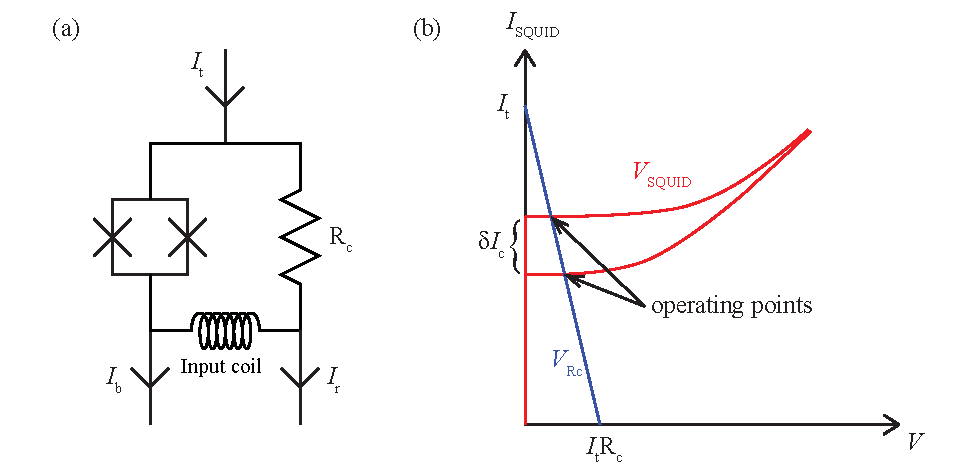
\includegraphics{experimental/Fig_loadline}\\
\caption[Bias and operating points of measured SQUID]{Bias and operating points of measured SQUID. (a) Simplified schematic of the typical biasing of a measured SQUID. (b) Current-voltage characteristics of a SQUID (red) for a small change in critical current. The load line for $R_c$ (blue) is calculated as follows. For zero current flowing through $R_c$, $V_{R_c} = 0$ and the current through the SQUID, $I_{\text{SQUID}}$, is maximum: $I_{\text{SQUID}} = I_t$. For $I_{\text{SQUID}} = 0$, the total current flows through $R_c$ and $V_{R_c} = I_t R_c$. The equilibrium solution occurs when $V_{\text{SQUID}} = V_{R_c}$, which is the intersection of the two curves. Therefore, $\delta I_c$ causes the operating points to change little in voltage, but maximally in current.}
\label{fig:experimental:loadline}
\end{figure}

% Optimization of Rc
In general, we choose parameters to maximize $\Vfll$ for a given change in critical current or flux in the measured SQUID. First, we discuss the value of the compensating resistor. In Fig.~\ref{fig:experimental:loadline}(a) we show a simplified schematic of the typical biasing of a SQUID, omitting the superconducting SQUIDs; here, $I_t = I_r + I_b$ is the total current applied to the circuit. Ultimately, we seek to maximize the change in current through the input coil for a given change in SQUID critical current. In this familiar circuit, we recognize that if $R_c \gg R_d$, the SQUID is effectively current biased. That is, if the critical current of the SQUID decreases slightly, $V_{\text{SQUID}}$ will increase by $\delta V$ and the current through $R_c$ will increase by only $\delta V/R_c$, which, by construct, is very small. However, if $R_c \ll R_d$, the SQUID is effectively voltage biased. We show this situation in Fig.~\ref{fig:experimental:loadline}(b), using the concept of load lines because the SQUID is a nonlinear circuit element. In this scenario, a decrease in $I_c$ of the SQUID corresponds to a maximum increase in increase of current through $R_c$ and, correspondingly, the input coil of the readout SQUID,
\begin{align}\label{fig:experimental:dIloop_dIc}
\Delta I_{\text{loop}} = \frac{1}{1+R_c/R_d} \Delta I_c.
\end{align}
For typical values of $R_d \sim 10~\Omega$, $R_c$ should be on the order of $1~\Omega$. Resistances much less than this value do not offer additional signal and can, in fact, degrade the performance if $R_c$ is too low.

% FLL and readout SQUID parameters
With a small value of $R_c$, we ensure that fluctuations in the readout SQUID generate maximum current fluctuations through the input coil of the readout SQUID. In turn, we maximize the flux coupled into the readout SQUID by using the largest feasible mutual inductance for the input coil $M_i$. In general, $M_i \sim 10~\text{nH}$, or $M_i^{-1} \sim 0.1~\mu\text{A}/\Phi_0$. Conversely, we aim to make the mutual inductance of the feedback coil $M_f$ small ($\sim 0.5~$nH) so that the feedback current is relatively large. Finally, the feedback resistor $R_{\text{feedback}}$, which sets the conversion factor between the feedback current and $\Vfll$, is chosen to be large ($\gtrsim 100~\text{k}\Omega$). Thus, the output of the FLL is related to the current in the loop $I_{\text{loop}}$ via
\begin{align}\label{fig:experimental:Vfll_Iloop}
\Vfll = R_{\text{feedback}} \left( \frac{M_i}{M_f} \right) I_{\text{loop}}.
\end{align}

% Optimization of junction parameters
It is also possible to optimize the junction parameters of the SQUIDs. By varying the value of the shunt resistance $R$ and critical current of the junctions, we can modify the level of white noise and flux sensitivity, respectively. At high enough frequencies---typically, above 10 to 100~Hz when the SQUID is biased at maximum flux sensitivity---the white noise generated by the shunt resistors becomes significant compared to the flux noise. As a current, the noise magnitude scales as $R^{-1}$~\citep{Likharev:1972}, which indicates that we can reduce the white noise level by increasing $R$. Because $\partial I_c/\partial\Phi$ is roughly proportional to $I_c$, we can also increase the sensitivity of our measurement to flux in the measured SQUID. These two criteria taken alone yield the prescription to increase $R$ and $I_c$ as much as possible. However, our measurements require that the SQUIDs operate non-hysteretically, that is, $\beta_c = 2\pi I_0 R^2 C/\Phi_0 < 1$~\citep{Stewart:1968,McCumber:1968}, so that $R$ and $I_c$ cannot be increased without bound. Here, $I_0 = I_c/2$ and $C$ are the average junction critical current and capacitance, respectively. For junction area $A$ and fixed current density $j_c$ and areal capacitance density $c$, $I_cR^2 C = (c/j_c)(j_c A)^2 R^2$, meaning the product $I_cR$ is fixed for constant $\beta_c$. Because the white noise decreases as $R^{-1}$ but the sensitivity increases as $(\partial I_c/\partial\Phi)^2 \propto I_c^2$, we see that it is most advantageous to increase $I_c$ as much as possible, even at the cost of decreasing $R$.

\section{Implementation}

\begin{figure}
\centering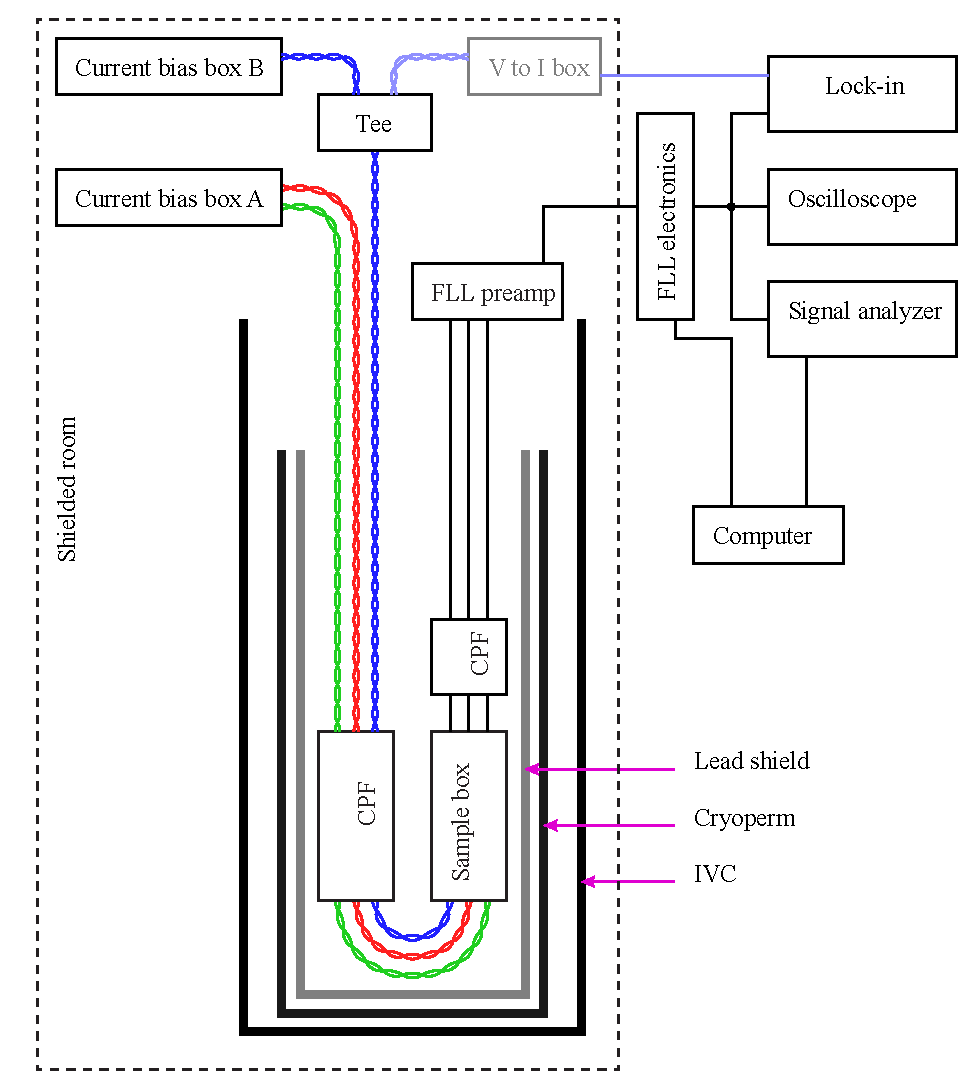
\includegraphics{experimental/Fig_meas_schematic}\\
\caption[Schematic of measurement system]{Schematic of measurement system. The sample is mounted to the cold finger of a dilution refrigerator and is surrounded by a combination shield of Pb and Cryoperm for magnetic shielding. All lines are low-pass filtered using copper powder filters (CPF) and discrete filters. The typical configuration of bias boxes and readout equipment is shown. The shaded portion is connected only when measuring $\partial I/\partial \Phi$, not when acquiring noise data. [@@@ This fig probably runs over the bottom margin! @@@ Add discrete filters]}
\label{fig:experimental:meas_schem}
\end{figure}

We now discuss the specifics of how we implement the measurement system, which is shown schematically in Fig.~\ref{fig:experimental:meas_schem}. The SQUIDs to be measured, which are typically fabricated on a single chip, are first mounted and wire-bonded onto a circuit board in one of the chambers of a copper sample box (Fig.~\ref{fig:experimental:sample_box}). Flux bias is provided either via an on-chip coil or a coil mounted in the circuit board, directly below the chip. The compensating resistor, which is simply a short segment of resistance wire, is also mounted to the circuit board. The readout SQUID is located in another chamber on the opposite side of the box in order to prevent cross-talk between SQUIDs. Intermediate chambers contain the choke inductor and the cold transformer of the readout SQUID. With the sample mounted, a lipped lid is attached. For magnetic shielding, the inner surfaces of both the box and lid are electroplated with approximately $200~\mu$m of Pb.

The sample box is then mounted onto the cold finger of an Oxford DR200 dilution refrigerator. In addition to the Pb plating of the sample box, further attenuation and shielding of external magnetic fields are provided by two concentric cans of Pb and Cryoperm. Electrical signals are carried via three 4-conductor Reichenbach cables for the various biasing of the measured SQUIDs and three SMA coaxial cables for the current bias, voltage readout, and flux feedback current of the readout SQUID. All lines are rf-filtered using standard copper powder filters (CPFs) and low-pass filtered using discrete filters. Bias currents are provided via lithium-ion battery-powered boxes using one of two circuit designs, shown in Fig.~\ref{fig:experimental:bias_boxes}. The current biases for $I_b$ and $I_r$ typically need to source only tens of microamps and use the ``passive'' design  [Fig.~\ref{fig:experimental:bias_boxes}(a)]. The current bias for the flux bias of the measured SQUIDs, however, can require in excess of 10~mA, so we use an ``active'' source [Fig.~\ref{fig:experimental:bias_boxes}(a)]. Both designs rely on the extremely flat discharge voltage of Li-ion batteries, which allows us to use them as simple, yet stable, voltage references. For the readout and control electronics of the FLL, we use two commercial packages available from Easy SQUID and STAR Cryoelectronics, respectively. Both packages come with amplification units that we attach directly atop the fridge. For additional isolation and electric shielding, the fridge and the electronics mentioned thus far are located within a shielded room, consisting of electrically continuous copper sheet (Fig.~\ref{fig:experimental:meas_schem}).

The FLL amplification box interfaces with the control electronics, external to the shielded room, via a filtered DB9 cable. The FLL control electronics in turn output $\Vfll$ and also connect to a computer, which provides control over the FLL parameters. The output $\Vfll$ is passed to a oscilloscope, which is used during the biasing procedure, as well as an Agilent~35670A signal analyzer. It is also passed to a lock-in amplifier that is used to measure $\partial I/\partial \Phi$, which is described in Section~\ref{chap:exp:sec:meas_proc}.

[@@@ anything else?]

\begin{figure}
\centering\includegraphics[width=6.5in]{experimental/sample_box.jpg}\\
\caption[Photo of sample box]{Photo of sample box. Six chambers separate the various portions of the measurement circuit. The circuit board holding the measured SQUIDs is on the left. On the right is the board holding the readout SQUID. The chambers in the middle hold the choke inductor and cold transformer, wound around molypermalloy powder (MPP) cores, which work well at cryogenic temperatures.}
\label{fig:experimental:sample_box}
\end{figure}

%\begin{figure}
%\centering\includegraphics[height=4in]{experimental/fridge.jpg}\\
%\caption{Picture of fridge}
%\label{fig:experimental:fridge_photo}
%\end{figure}

\begin{figure}
\centering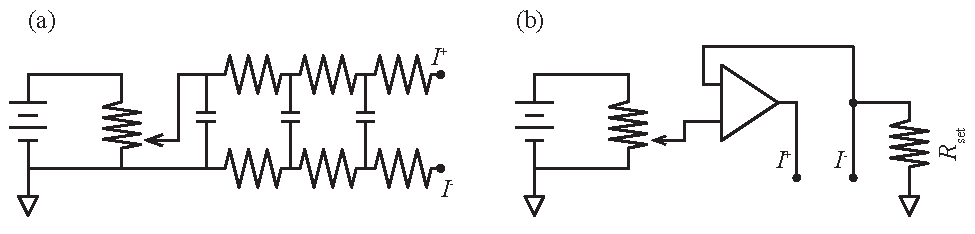
\includegraphics{experimental/Fig_current_supplies}\\
\caption[Circuit schematics of current supply boxes]{Circuit schematics of current supply boxes. (a) ``Passive'' circuit design, type A. Li-ion battery sources a current controlled by a 10-turn potentiometer. This design is useful for sourcing $\lesssim 100~\mu$A. (b) ``Active'' circuit design, type B. The Li-ion battery and 10-turn potentiometer provide a stable voltage source input to the op-amp (ISL28134). $R_{\text{set}}$ sets the current output range, which, for this op-amp, is approximately $60~\mu$A. Since the op-amp sources the current, the discharge on the Li-ion batter is minimal.}
\label{fig:experimental:bias_boxes}
\end{figure}

\section{Calibration and validation}

In order to validate the system, we must first measure certain parameters in order to calibrate conversion factors and then verify that the readout and bias electronics are sufficiently low-noise. First, we seek to calibrate the output of the FLL; that is, we want to know $\partial\Iloop/\partial\Vfll$. From Eq.~\eqref{fig:experimental:Vfll_Iloop}, this means we need to measure $M_i$, $M_f$, and $R_{\text{feedback}}$. There is a trick, however, that allows a direct calibration of $\partial\Vfll/\partial\Phi_a$, where $\Phi_a$ is the flux in the readout SQUID. Then,
\begin{align}\label{fig:experimental:dIloop_dVfll}
\frac{\partial\Iloop}{\partial\Vfll} = \left(\frac{\partial\Iloop}{\partial\Phi_a}\right) \left(\frac{\partial\Phi_a}{\partial\Vfll}\right) %
= M_i^{-1} \left(\frac{\partial\Vfll}{\partial\Phi_a}\right)^{-1}.
\end{align}
We begin by locking the FLL with zero current in the big loop and recording the voltage. Next, we unlock the loop, inject a current into the input coil corresponding to approximately one flux quantum, and lock the loop. We can do this even with the SQUIDs bonded into the loop by injecting current across the compensating resistor ($I_r$). Since the SQUIDs are superconducting, the current will flow through the lowest resistance path; that is, all the current will flow through the SQUIDs and input coil. With the loop locked, we now reduce the bias current back to zero and again record $\Vfll$. The difference in recorded voltages $\Delta \Vfll$ corresponds to one $\Phi_0$ in the readout SQUID, $\partial\Vfll/\partial\Phi_a = \Delta \Vfll / \Phi_0$, which is about 0.5~V/$\Phi_0$ for our system. This method is described in detail in Sec.~2.10a of Ref.~\citep{Wellstood:thesis}. The mutual inductance of the input coil $M_i$ can be readily measured by injecting a known bias current into the circuit---again, across the compensating resistor if SQUIDs are in the circuit---and measuring $\Vfll$. For $M_i \approx 10$~nH, $\partial\Iloop/\partial\Vfll \approx 0.4~\mu$A/V.

Next, we must calibrate $\Vfll$ to changes in the measured SQUID. Changes in $I_c$ are related to $\Vfll$ via
\begin{align}\label{fig:experimental:dIc_dVfll}
\frac{\partial I_c}{\partial\Vfll} = \left(\frac{\partial I_c}{\partial\Iloop}\right) \left(\frac{\partial\Iloop}{\partial\Vfll}\right) %
\approx \frac{\partial\Iloop}{\partial\Vfll}
\end{align}
by Eq.~\eqref{fig:experimental:dIloop_dIc} for $R_c \ll R_d$. For our applications, Eq.~\eqref{fig:experimental:dIc_dVfll} is sufficiently accurate---10\% for $R_c = R_d/10$---as we are not focused on highly accurate measurements of critical current noise. To scale $\Vfll$ to an equivalent flux noise, we measure the change $\Delta\Vfll$ in response to a known applied flux in the measured SQUID $\Delta\Phi_m$, which is described in the next Section.

After establishing the relevant conversion factors, we want to characterize the noise of the measurement system. With the measured SQUIDs in the superconducting state, the major sources of noise are (i) the amplification and readout electronics of the FLL, (ii) the intrinsic critical current and flux noise of the readout SQUID, and (iii) the Nyquist noise of the compensating resistor~\citep{Nyquist:PR:1928}. While it is possible to measure the noise from (i) and (ii) independently, the characterization process is complicated, lengthy, and involves several cooldowns to 4~K. A much simpler method exists that puts an upper bound on the combined noise of (i) and (ii). With accurate knowledge of the compensating resistance $R_c$ and temperature $T$, we can calculate the Nyquist current noise spectral density as $S_{I,R_c} = 4 k_B T/R_c$. By comparing the measured to predicted noise, we can estimate the noise added by the readout. In addition, we can confirm the calibration of the system. We find that our electronics add approximately $3~(\text{pA})^2$/Hz of white noise, which is negligible compared to $S_{I,R_c}$ for $T \gtrsim 0.3$~K and $R_c \approx 0.5~\Omega$. Above this temperature, agreement between measurement and prediction is better than 10\%.




\section{Measurement procedure}\label{chap:exp:sec:meas_proc}




\section{Low-frequency critical current noise}










